\subsubsection{Arbre de décision}

L'arbre de décision (fig \ref{fig:ArbreDecision}), qui permet de localiser le bâtiment contenant un point donné, est composé d'un noeud racine qui se découpe en quatre noeuds par rapport à son centre, qui se découpent également chacun en quatre noeuds par rapport à leur centre, jusqu'à atteindre les feuilles.\\

Un noeud est représenté par la classe \texttt{Node}, et une feuille par la classe \texttt{Leaf}. Ces deux classes implémentent l'interface \texttt{INode} qui propose la méthode de localisation du point \texttt{BoundingBox locate(double x, double y)}. Comme la classe \texttt{BoundingBox} est utilisée pour stocker le rectangle englobant et l'identifiant d'un bâtiment, on peut considérer que la méthode \texttt{locate} retourne le bâtiment contenant le point donné. Le rectangle englobant est tout simplement le plus petit rectangle contenant l'ensemble des points du polygone formant le bâtiment.\\

Un noeud contient des coordonnées \texttt{x} et \texttt{y}, qui correspondent à son centre, et les quatre sous-noeuds qui le composent. Ces coordonnées servent à savoir où se situe le point donné par rapport au centre du noeud, et si il faut appeler la méthode \texttt{locate} sur le sous-noeud en haut à gauche, en haut à droite, en bas à gauche, ou en bas à droite.

Une feuille contient la liste des bâtiments dont le rectangle englobant intersecte sa zone. Par exemple, si l'arbre couvre une zone dont le point en haut à gauche est $(0, 0)$, et le point en bas à droite est $(1, 1)$, et qu'il possède un noeud racine qui se décompose en quatre feuilles, alors le centre du noeud est le point $(0.5, 0.5)$, et la feuille en haut à gauche contient la liste des bâtiments dont le rectangle englobant intersecte le rectangle d'origine $(0, 0)$, de largeur $0.5$, et de hauteur $0.5$.\\

Avec cette structure, au lieu de devoir tester tous les bâtiments existants, on commence par récupérer la feuille qui contient le point, et ainsi, on est sûr de ne tester que les bâtiments qui intersectent la zone représentée par la feuille et qui ont une chance de contenir le point. De plus, on ne teste pas si un bâtiment contient le point par rapport au polygone qui représente le bâtiment, mais par rapport à son rectangle englobant.

\`{A} noter que si une une feuille ne contient aucun bâtiment, alors elle remplacée par \texttt{NullNode.NULL} dans l'arbre. De même, si les quatre sous-noeuds d'un noeud correspondent à \texttt{NullNode.NULL}, alors le noeud est remplacé par \texttt{NullNode.NULL}. Ainsi, un noeud n'existe dans l'arbre que si il possède au moins une feuille qui contient des bâtiments. Par conséquent, l'arbre prend considérablement moins de place en mémoire, et la localisation d'un point s'arrête immédiatement si le point se situe dans une zone sans bâtiments.

\begin{figure}[h!]
\centering
\resizebox{0.75\linewidth}{!}{
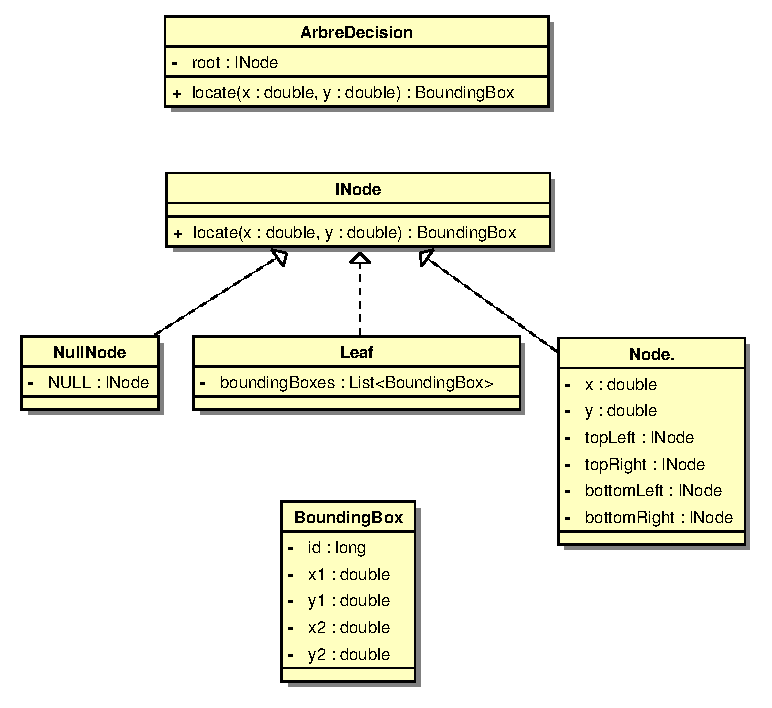
\includegraphics[width=1\textwidth]{../images/modeleArbreDecision.pdf}
}
\label{fig:ArbreDecision}
\caption{Arbre de décision}
\end{figure}